\documentclass[12pt]{scrbook}

\usepackage{epsfig}
\usepackage{a4wide}
\usepackage{times}
\usepackage{fancyhdr}

\sloppy
% page headings

\pagestyle{fancyplain}
\renewcommand{\chaptermark}[1]{\markboth{#1}{#1}}
\renewcommand{\sectionmark}[1]{\markright{\thesection\ #1}}
\lhead[\sf\bfseries\fancyplain{}{\thepage}]{\sf\fancyplain{}{\rightmark}}
\rhead[\sf\fancyplain{}{\leftmark}]{\sf\bfseries\fancyplain{}{\thepage}}
\cfoot{}

\title{JacORB 1.3 Programming Guide}

\author{Gerald Brose, Nicolas Noffke, Sebastian M\"uller\\
Institut f\"ur Informatik\\
Freie Universit\"at Berlin, Germany\\
\{brose,noffke,semu\}@inf.fu-berlin.de\\
\\
$Revision: 1.5 $
}

\begin{document}

% uniform formatting of a command line, includes leading $
\newcommand{\cmdline}[1]{\begin{small}\noindent \texttt{\$ #1}\end{small}}

\maketitle


\setlength{\parskip}{1.1ex}
\newpage
\tableofcontents

\chapter{Introduction}

This  document  gives   an  introduction  to  programming  distributed
applications with  JacORB, a free  Java object request  broker. JacORB
comes  with  full  source  code,  a couple  of  CORBA  Object  Service
implementations, and  a number of example programs.   This document is
{\it  not}   an  introduction  to   CORBA  in  general.    Please  see
\cite{Brose2001a,Siegel2000,   Vinoski1997}  for   this   purpose  and
\cite{Henning1999}  for  more  advanced  issues.  The  JacORB  version
described in this document is JacORB 1.3. This document is intended to
give a  few essential hints on how  to install and use  JacORB, but it
will  not  suffice as  either  a gentle  introduction  to  CORBA or  a
tutorial.

%%%%%%%%%%%%%%%%%%%%%%%%%%%%%%%%%%%%%%%%%%%%%%%%%%%%%%%%%%%%%%%%%%%%%%%%%%%%%%

\chapter{Installing JacORB}
\label{Ch_installing}

In this chapter  we explain how to obtain and  install JacORB and give
an overview of the package contents.

\section{Obtaining JacORB}

JacORB can be obtained as a g-zipped tar--archive or as a zip--archive
from the  JacORB home page  at \verb+http://jacorb.inf.fu-berlin.de/+.
It   can   also   be   downloaded   via  anonymous   ftp   from   {\tt
ftp.inf.fu-berlin.de} from the directory {\tt pub/jacorb/}.

To install JacORB, just unzip  and untar (or simply unzip) the archive
somewhere.   This will  result in  a new  directory  {\tt JacORB1\_3}.
Make   sure  your   CLASSPATH  environment   variable   contains  {\tt
JacORB1\_3/lib/jacorb.jar}.  If you plan  to recompile all or parts of
JacORB, you should also include {\tt JacORB1\_2/classes}.  Extend your
search path with  {\tt JacORB1\_3/bin}, so that the  shell scripts and
batch files for the utilities in this directory are found.

\section{Installation}
\label{Sec_installation}

\subsection{Ant and build files}

JacORB will run on any JavaVM,  but to rebuild JacORB (and compile the
 examples) you need to have the XML--based make tool ``Ant'' installed
 on    your   machine.    Ant    can   be    downloaded   from    {\tt
 http://jakarta.apache.org/ant}. All make  files ({\tt build.xml}) are
 written for this  tool. To rebuild JacORB completely,  just type {\tt
 ant} in the installation directory.  Optionally, you might want to do
 a {\tt ant clean} first.

In order to be able to  use GUI tools such as NameManager, ImRManager,
IRBrowser, and  the KeyStoreManager, you need  to use JDK  1.2 or have
Sun's Swing  classes installed on  your machine.  In the  latter case,
your CLASSPATH also needs to  contain these classes. For SSL, you must
have  JDK 1.2.  Also, you  need to  install the  cryptography  and SSL
libraries by  IAIK, viz.  IAIK--JCE  2.5 and iSaSiLk 3.0.   Please see
{\tt http://jcewww.iaik.tu-graz.ac.at/}.

\subsection{Configuration}

JacORB has a number of configuration  options which can be set as Java
properties.  Before we will go about explaining some of the more basic
options   here,  let's  look   at  the   different  ways   of  setting
properties. Specific  options that apply, e.g.,  to the Implementation
Repository  or  the  Trading  Service  are explained  in  the  chapter
discussing these modules. There are three options for doing this.

The most  general case is in  a properties file. JacORB  looks for and
loads  a   file  called  either  {\tt   .jacorb\_properties}  or  {\tt
jacorb.properties}.   It  looks for  these  files  in  both your  home
directory  (as in  the {\tt  user.home}  system property)  and in  the
current directory.  If  it finds multiple files, it  loads all of them
in this  order. In case of  different settings for  the same property,
the one loaded last takes precedence.

For  more  application--specific  properties,  you  can  pass  a  {\tt
java.util.Properties}  object to  {\tt ORB.init()}  during application
initialization,  e.g.,  like this  ({\tt  args}  is  the String  array
containing command line arguments):

\small{
\begin{verbatim}            
    java.util.Properties props = new java.util.Properties();
    props.setProperty("jacorb.implname","StandardNS"); // use put() under Java 1.1
    org.omg.CORBA.ORB orb = org.omg.CORBA.ORB.init(args, props);
\end{verbatim}
}

The third way  of specifying properties is by  passing them as command
line  arguments   to  the  Java  interpreter.  This   option  has  the
disadvantage  that  you cannot  use  {\tt  jaco}  to start  the  Java
interpreter, which  means that  you must pass  in the  properties that
this script sets.

\cmdline{java -DOAPort=4711 -D... -D... jacorb.naming.NameServer ...}

An option  passed like  this will override  any setting in  either the
properties  file  or the  application  setup.  Properties  set in  the
application code, however, will  always override any properties set in
any other way.

We are now ready to have a look at the most basic JacORB configuration
properties.  Here is an example {\tt jacorb\_properties} file: 

\renewcommand{\baselinestretch}{0.9}
\small{
\begin{verbatim}
##
##  JacORB configuration options
##

########################################
#                                      #
#   Initial references configuration   #
#                                      #
########################################

#
# URLs where IORs are stored (used in orb.resolve_initial_service())
# DO EDIT these! (Only those that you are planning to use,
# of course ;-). 
#
# The ORBInitRef references are created on ORB startup time. In the 
# cases of the services themselves, this may lead to exceptions being 
# displayed (because the services aren't up yet). These exceptions
# are handled properly and cause no harm! 

#ORBInitRef.NameService=corbaloc::160.45.110.41:38693/\
#                       StandardNS/NameServer%2DPOA/_root
#ORBInitRef.NameService=file:/c:/NS_Ref
ORBInitRef.NameService=http://www.x.y.z/~user/NS_Ref
#ORBInitRef.TradingService=http://www.x.y.z/~user/TraderRef

# JacORB-specific URLs
jacorb.ImplementationRepositoryURL=http://www.x.y.z/~user/ImR_Ref
jacorb.ProxyServerURL=http://www.x.y.z/~user/Appligator_Ref

##################################
#                                #
#   Debug output configuration   #
#                                #
##################################

# use (java) jacorb.util.CAD to generate an appropriate
# verbosity level 
# 0 = off
# 1 = important messages and exceptions
# 2 = informational messages and exceptions
# >= 3 = debug-level output (may confuse the unaware user :-)
jacorb.verbosity=1

# where does output go? Terminal is default
#jacorb.logfile=LOGFILEPATH

##################################################
#                                                #
#    WARNING: The following properties should    # 
#    only be edited by the expert user. They     #
#    can be left untouched for most cases!       #
#                                                #
##################################################

################################
#                              #
#   Basic ORB Configuration    #
#                              #
################################

# number of retries if connection cannot directly be established
jacorb.retries=5

# how many msecs. do we wait between retries
jacorb.retry_interval=500

# size of network buffers for outgoing messages
jacorb.outbuf_size=2048

# client-side timeout, set no non-zero to stop blocking
# after so many msecs.
#jacorb.connection.client_timeout=0

# max time a server keeps a connection open if nothing happens
#jacorb.connection.server_timeout=10000

#jacorb.reference_caching=off
...

#########################
#                       #
#   POA Configuration   #
#                       #
#########################

# displays a GUI monitoring tool for servers
jacorb.poa.monitoring=off

# thread pool configuration for request processing
jacorb.poa.thread_pool_max=20
jacorb.poa.thread_pool_min=5

# if set, request processing threads in thePOA
# will run at this priority. If not set or invalid,
# MAX_PRIORITY will be used.
#jacorb.poa.thread_priority=

# size of the request queue, clients will receive Corba.TRANSIENT
# exceptions if load exceeds this limit
jacorb.poa.queue_max=100
...
\end{verbatim}
}
\renewcommand{\baselinestretch}{1.0}
\small\normalsize

Configurable options  include the size of network  buffers, the number
of retries JacORB makes if a connection cannot be established, and how
long  it  shall wait  before  retrying.   The  string value  for  {\tt
ORBInitRef.NameService} is  a URL  for a resource  used to set  up the
JacORB name  server. This URL  will be used  by the ORB to  locate the
file  used to  store  the  name server's  object  reference (see  also
chapter \ref{names}).

The {\tt verbosity} option tells  JacORB how much diagnostic output it
should emit at runtime. Unless the  {\tt logfile} property is set to a
file name, diagnostic output will  be sent to the terminal. Setting the
verbosity property to 0 means don't print any, while a level of 2 is a
verbose debug mode.   Level 1 will emit some  information, e.g.  about
connections  being  opened,  accepted  and  closed.  If  you  like  to
selectively  suppress  specific  output  you  can  use  the  tool  {\tt
jacorb.util.CAD} to generate a special verbosity level.

The  {\tt jacorb.poa.monitoring} property  determines whether  the POA
should bring up a monitoring GUI  for servers that let you examine the
dynamic behavior of  your POA, e.g.  how long  the request queue gets
and whether your thread pool is  big enough.  Also, this tool lets you
change the  state of a POA,  e.g. from {\it active}  to {\it holding}.
Please see chapter \ref{POA} on the POA for more details.

You can now test your installation  by typing {\tt ant} in one of the
subdirectories of the {\tt demo/} directory which contains a number of
examples for using JacORB.
    
%%%%%%%%%%%%%%%%%%%%%%%%%%%%%%%%%%%%%%%%%%%%%%%%%%%%%%%%%%%%%%%%%%%%%%%%%%%%%%

\chapter{Getting Started}
\label{start}

Before we  explain an example  in detail, we  will have a look  at the
general process  of developing  CORBA applications with  JacORB. We'll
follow this roadmap when working through the example.  The example can
be found in  {\tt demo/grid} which also contains a  build file so that
the development  steps do  not have to  be carried out  manually every
time.  Still, you should know what is going on.

As this document gives only a short introduction to JacORB programming
and does not cover all the details of CORBA IDL, we recommend that you
also look at  the other examples in the  {\tt demo/} directory.  These
are organized so as to show how the different aspects of CORBA IDL can
be used with JacORB.

\section{JacORB development: an overview}

The steps we will generally have to take are:

\begin{enumerate}
    \item  write an IDL specification.
    \item  compile this specification with the IDL compiler to generate Java classes.
    \item write an implementation for the interface generated in step
      2
    \item  write a ``Main'' class that instantiates the server implementation
        and registers it with the ORB
    \item  write a client class that retrieves a reference to the server object.
\end{enumerate}


\section{IDL specifications}

Our example uses a simple server the definition of which should be
clear if you know IDL. Its interface is given in {\tt server.idl}. All
the source code for this example can be found in {\tt
  JacORB1\_3/demo/grid}.

\small{
\begin{verbatim}
// server.idl
// IDL definition of a 2-D grid:
module demo
{
  module grid 
  { 
    interface MyServer
    {
        typedef fixed <5,2> fixedT;

        readonly attribute short height;  // height of the grid
        readonly attribute short width;   // width of the grid

        // set the element [n,m] of the grid, to value:
        void set(in short n, in short m, in fixedT value);

        // return element [n,m] of the grid:
        fixedT get(in short n, in short m);
        
        exception MyException
        {
            string why;
        };

        short opWithException() raises( MyException );
    };
  };
};
\end{verbatim}
}

\section{Generating Java classes}

Feeding this file into the IDL compiler 

\cmdline{idl -d ../..  server.idl}

produces a number of Java  classes that represent the IDL definitions.
This is  done according to a  set of rules known  as the IDL--to--Java
language mapping as standardized by  the OMG. If you are interested in
the details of the language mapping, i.e. which IDL language construct
is  mapped  to  which  Java  language construct,  please  consult  the
specifications available from  {\tt www.omg.org}. The language mapping
used by the JacORB IDL compiler is the one defined in CORBA 2.3 and is
explained in detail in  \cite{Brose2001a}. For practical usage, please
consult the examples in the {\tt demo} directory.

The most important Java classes  generated by the IDL compiler are the
interfaces {\tt  MyServer} and {\tt MyServerOperations}  plus the stub
and  skeleton   files  {\tt  \_MyServerStub,   MyServerPOA}  and  {\tt
MyServerPOATie}.  We will  use these classes in the  client and server
as  well as  in the  implementation  of the  grid's functionality  and
explain each in turn.

Note that the IDL compiler  will produce a directory structure for the
generated code  that corresponds  to the module  structure in  the IDL
file, so it would have  produced a subdirectory {\tt demo/grid} in the
current  directory  had we  not  directed  it  to put  this  directory
structure  to {\tt  ../..} by  using the  compiler's {\tt  -d} switch.
Where to  put the source  files for generated  classes is a  matter of
taste.  Some people  prefer to have everything in  one place (as using
the {\tt  -d} option in  this way achieves),  others like to  have one
subdirectory for the generated source  code and another for the output
of the Java compiler, i.e. for the {\tt .class} files.


\section{Implementing the interface}

Let's try  to actually provide an implementation  of the functionality
promised by  the interface. The class which  implements that interface
is called {\tt gridImpl}.   Apart from providing a Java implementation
for the operations listed in the IDL interface, it has to inherit from
a generated class that both  defines the Java type that represents the
IDL type {\tt MyServer} and contains the code needed to receive remote
invocations and return results to  remote callers.  This class is {\tt
MyServerPOA}.

You might have noticed that this approach is impractical in situations
where your  implementation class needs to inherit  from other classes.
As  Java only has  single inheritance  for implementations,  you would
have  to use  an alternative  approach ---  the  ``tie''--approach ---
here. The tie approach will be explained later.

Here is  the Java code for  the grid implementation. It  uses the Java
library  class  {\tt  java.math.BigDecimal}  for  values  of  the  IDL
fixed--point type {\tt fixedT}:

\small{
\begin{verbatim}
package demo.grid;

/**
 * A very simple implementation of a 2-D grid
 */

import demo.grid.MyServerPackage.MyException;

public class gridImpl  
    extends MyServerPOA
{
    protected short height = 31;
    protected short width = 14;
    protected java.math.BigDecimal[][] mygrid;
 
    public gridImpl()
    {
        mygrid = new java.math.BigDecimal[height][width];
        for( short h = 0; h < height; h++ )
        {
            for( short w = 0; w < width; w++ )
            {
                mygrid[h][w] = new java.math.BigDecimal("0.21");
            }
        }
    }

    public java.math.BigDecimal get(short n, short m)
    {
        if( ( n <= height ) && ( m <= width ) )
            return mygrid[n][m];
        else
            return new java.math.BigDecimal("0.01");
    }

    public short height()
    {
        return height;
    }

    public void set(short n, short m, java.math.BigDecimal value)
    {
        if( ( n <= height ) && ( m <= width ) )
            mygrid[n][m] = value;
    }

    public short width()
    {
        return width;
    }

    public short opWithException()
        throws demo.grid.MyServerPackage.MyException
    {
        throw new demo.grid.MyServerPackage.MyException("This is only a test exception, no harm done :-)");
    }
}
\end{verbatim}
}

\section{Writing the Server}

To actually instantiate a {\tt  gridImpl} object which can be accessed
remotely  as  a CORBA  object  of type  {\tt  MyServer},  you have  to
instantiate it  in a main method  of some other class  and register it
with a  component of the CORBA  architecture known as  the {\it Object
Adapter}. Here is  the class {\tt Server} which  does all that is
necessary to  activate a  CORBA object of  type {\tt MyServer}  from a
Java {\tt gridImpl} object:

\small{
\begin{verbatim}
package demo.grid;

import java.io.*;
import org.omg.CosNaming.*;

public class Server
{
    public static void main( String[] args )
    {
        org.omg.CORBA.ORB orb = org.omg.CORBA.ORB.init(args, null);
        try
        {
            org.omg.PortableServer.POA poa = 
                org.omg.PortableServer.POAHelper.narrow(
                     orb.resolve_initial_references("RootPOA"));
            
            poa.the_POAManager().activate();

            org.omg.CORBA.Object o = poa.servant_to_reference(new gridImpl());

            if( args.length == 1 ) 
            {
                // write the object reference to args[0]

                PrintWriter ps = new PrintWriter(
                                    new FileOutputStream(
                                       new File( args[0] )));
                ps.println( orb.object_to_string( o ) );
                ps.close();
            } 
            else
            {
                // register with the naming service             

                NamingContextExt nc = 
                     NamingContextExtHelper.narrow(
                        orb.resolve_initial_references("NameService"));
                nc.bind( nc.to_name("grid.example"), o);        
            }
        } 
        catch ( Exception e )
        {
            e.printStackTrace();
        }
        orb.run();
    }
}
\end{verbatim}
}

After initializing the ORB we need to obtain a reference to the object
adapter --- the POA --- by asking  the ORB for it. The ORB knows about
a few initial references that can be retrieved using simple names like
``RootPOA''. The returned object is  an untyped reference of type {\tt
CORBA.Object} and thus needs to  be narrowed to the correct type using
a static  method {\tt narrow()}  in the helper  class for the  type in
question. We now  have to activate the POA because  any POA is created
in  ``holding''   state  in  which   it  does  not   process  incoming
requests.  After  calling {\tt  activate()}  on  the POA's  POAManager
object, the POA is in an active state and can now be asked to create a
CORBA  object  reference  from a  Java  object  also  know as  a  {\tt
Servant}.

In order to make the newly created CORBA object accessible, we have to
make its  object reference  available. This is  done using  a publicly
accessible directory  service, the naming  server. A reference  to the
naming      service     is      obtained      by     calling      {\tt
orb.resolve\_initial\_references("NameService")}   on   the  ORB   and
narrowing the reference using the {\tt narrow()} method found in class
{\tt org.omg.CosNaming.NamingContextExtHelper}.  Having done this, you
should call the  {\tt bind()} operation on the  name server.  The name
for the object which has to be supplied as an argument to {\tt bind()}
is not simply a string. Rather, you need to provide a sequence of {\tt
CosNaming.NameComponent}s that represent the  name. In the example, we
chose to use an extended Name Server interface that provides us with a
more convenient conversion operation from strings to Names.


\section{Writing a client}

Finally, let's have a look at the client class which invokes the
server operations:

\small{
\begin{verbatim}
package demo.grid;

import org.omg.CosNaming.*;

public class Client
{
   public static void main(String args[]) 
   { 
       try
       {
           MyServer grid;
           org.omg.CORBA.ORB orb = org.omg.CORBA.ORB.init(args,null);

           if(args.length==1 )
           {
               // args[0] is an IOR-string 
               grid = MyServerHelper.narrow(orb.string_to_object(args[0]));
           }
           else
           {
               NamingContextExt nc =
                   NamingContextExtHelper.narrow(
                      orb.resolve_initial_references("NameService"));

               grid = MyServerHelper.narrow(
                         nc.resolve(nc.to_name("grid.example")));
            }

            short x = grid.height();
            System.out.println("Height = " + x);

            short y = grid.width();
            System.out.println("Width = " + y);

            x -= 1;
            y -= 1;

            System.out.println("Old value at (" + x + "," + y +"): " + 
                               grid.get( x,y));

            System.out.println("Setting (" + x + "," + y +") to 470.11");
                
            grid.set( x, y, new java.math.BigDecimal("470.11"));

            System.out.println("New value at (" + x + "," + y +"): " + 
                               grid.get( x,y));

           try 
           {
               grid.opWithException();
           }
           catch (jacorb.demo.grid.MyServerPackage.MyException ex) 
           {
               System.out.println("MyException, reason: " + ex.why);
           }
       }
       catch (Exception e) 
       {
           e.printStackTrace();
       }
   }
}
\end{verbatim}
}

After  initializing the  ORB, the  client obtains  a reference  to the
``grid''  service by locating  the reference  using the  name service.
Again, resolving the name is done by getting a reference to the naming
service                 by                 calling                {\tt
orb.resolve\_initial\_references("NameService")} and querying the name
server for  the {\tt "grid"}  object by calling {\tt  resolve()}.  The
argument  to  the  resolve  operation  is, again,  a  string  that  is
converted to  a Name. The result  is an object reference  of type {\tt
org.omg.CORBA.Object}  which has  to be  narrowed to  the type  we are
expecting, i.e. {\tt MyServer}.

After compiling everything we're now  ready to actually run the server
and the  client on  different (virtual) machines.  Make sure  the name
server is running before starting  either the server or the client. If
it isn't, type something like:

\cmdline{ns /home/me/public\_html/NS\_Ref}
    
where  {\tt /home/me/public\_html/NS\_Ref}  is the  name of  a locally
writable file  which can be  read by using  the URL given in  both the
remote client and  server code. (This is to  avoid using a well--known
address for  the name server,  so both client  and server look  up the
location of the  name server via the URL and  later communicate with it
directly.)
    
You can now launch the server:

\cmdline{jaco demo.grid.Server}

The client can be invoked on any machine you like:

\cmdline{jaco demo.grid.Client}
    
Running the  client after starting  the server produces  the following
output on your terminal:

\begin{verbatim}
Height = 31
Width = 14
Old value at (30,13): 0.21
Setting (30,13) to 470.11
New value at (30,13): 470.11
MyException, reason: This is only a test exception, no harm done :-)
done.
\end{verbatim}

\subsection{The Tie Approach}

If your implementation class cannot inherit from the generated servant
class  {\tt  MyServerPOA} because,  e.g.,  you  need  to inherit  from
another  base class,  you can  use the  tie approach.  Put  simply, it
replaces  inheritance by  delegation. Instead  of inheriting  from the
generated  base  class, your  implementation  needs  to implement  the
generated {\em operations interface} {\tt MyServerOperations}:

\begin{verbatim}
package demo.grid;

import demo.grid.MyServerPackage.MyException;

public class gridOperationsImpl  
    implements MyServerOperations
{
...
}
\end{verbatim}

Your server is then written as follows:

\begin{verbatim}
package demo.grid;

import java.io.*;
import org.omg.CosNaming.*;

public class TieServer
{
    public static void main( String[] args )
    {
        org.omg.CORBA.ORB orb = 
            org.omg.CORBA.ORB.init(args, null);
        try
        {
            org.omg.PortableServer.POA poa = 
                org.omg.PortableServer.POAHelper.narrow(
                     orb.resolve_initial_references("RootPOA"));

            // use the operations implementation and wrap it in
            // a tie object

            org.omg.CORBA.Object o = 
                poa.servant_to_reference( 
                     new MyServerPOATie( new gridOperationsImpl()) );

            poa.the_POAManager().activate();

            if( args.length == 1 ) 
            {
                // write the object reference to args[0]

                PrintWriter ps = new PrintWriter(
                    new FileOutputStream(new File( args[0] )));
                ps.println( orb.object_to_string( o ) );
                ps.close();
            } 
            else
            {
                NamingContextExt nc = 
                     NamingContextExtHelper.narrow(
                        orb.resolve_initial_references("NameService"));
                NameComponent [] name = new NameComponent[1];
                name[0] = new NameComponent("grid", "whatever");
                nc.bind( name, o );
            }
        } 
        catch ( Exception e )
        {
            e.printStackTrace();
        }
        orb.run();
    }
}
\end{verbatim}




%%%%%%%%%%%%%%%%%%%%%%%%%%%%%%%%%%%%%%%%%%%%%%%%%%%%%%%%%%%%%%%%%%%%%%%%%%%%%%

\chapter{The JacORB Name Service}
\label{names}

Name  servers  are used  to  locate  objects  using a  human--readable
reference (their  name) rather than  a machine or network  address. If
objects providing  a certain service  are looked up using  the service
name, their  clients are  decoupled from the  actual locations  of the
objects that provide  this service.  The binding from  name to service
can be changed without the clients needing to know.

JacORB provides  an implementation  of the OMG's  Interoperable Naming
Service  which supports  binding  names to  object  references and  to
lookup object references using these names.  It also allows clients to
easily  convert names  to  strings  and vice  versa.  The JacORB  name
service comprises two  components: the name server program,  and a set
of interfaces and classes used to access the service.

One word  of caution about using  JDK 1.2 (and above)  with the JacORB
naming service: JDK 1.2 comes with a couple of outdated and apparently
buggy naming service classes that do not work properly with JacORB. To
avoid having these classes  loaded and used inadvertently, please make
sure that  you always use the {\tt  NamingContextExt} interface rather
than the plain {\tt  NamingContext} interface in your code. Otherwise,
you  will   see  your  application  receive  null   pointer  or  other
exceptions. Note that there is no such problem with JDK 1.1.

\section{Running the Name Server}

The JacORB  name server is a  process that needs to  be started before
the name service can be accessed by programs. Starting the name server
is done by typing on the command line either simply

\cmdline{ns <ior filename> [<timeout>]}

You can also start the Java interpreter explicitly by typing

\cmdline{jaco jacorb.naming.NameServer <filename> [<timeout>]}

In the example

\cmdline{ns /home/me/public\_html/NS\_Ref}

we direct  the name server  process to write location  information and
logging information to  the file {\tt /home/me/public\_html/NS\_Ref}.  A
client--side ORB uses this file to locate the name server process. The
client--side ORB does not, however, access the file through a local or
shared file  system by  default.  Rather,  the file is  read as  a WWW
resource by  using a URL pointing  to it.  This implies  that the name
server log file is accessible through  a URL in the first place, i.e.,
that you  know of a  web server in  your domain which can  answer HTTP
request to read the file.

The advantage of this approach is  that clients do not need to rely on
a hard--coded well known port  and that the name server is immediately
available world--wide  if the URL uses  HTTP. If you  want to restrict
name server visibility  to your domain (assuming that  the log file is
on a shared  file system accessible throughout your  domain) or you do
not have  access to a  web server, you  can use file URLs  rather than
HTTP URLs,  i.e. the URL pointing  to your name server  log file would
looks like

\noindent{\tt file:/home/brose/public\_html/NS\_Ref}

rather than 

\noindent\verb+http://www.inf.fu-berlin.de/~brose/NS_Ref+

Specifying file URLs  is also useful on machines  that have no network
connection at all. Please note that the overhead of using HTTP is only
incurred  once ---  when the  clients  first locate  the name  server.
Subsequent  requests  will use  standard  CORBA operation  invocations
which means they will be IIOP requests (over TCP).

The name server stores its  internal state, i.e., the name bindings in
its context,  in files  in the current  directory unless  the property
{\tt jacorb.naming.db\_dir} is set to a different directory name. This
saving is done  when the server goes down  regularly, i.e. killing the
server  with CTRL-C  will result  in loss  of data.   The  server will
restore state from its files if any files exist and are non--empty.

The second  parameter is a time--out  value in msecs. If  this value is
set, the name server will shut down after the specified amount of time
and save  its state. This is  useful if the name  server is registered
with  the  Implementation Repository  and  can  thus  be restarted  on
demand.

\subsection*{Configuring a Default Context}

Configuring a naming context (i.e. a name server) as the ORB's default
or root context is done by  simply writing the URL that points to this
server's    bootstrap    file   to    the    properties   file    {\tt
.jacorb\_properties}.  Alternatively,  you can  set this file  name in
the property {\tt ORBInitRef.NameService} either on the command line or
within the application  as described in \ref{Sec_installation}.  After
the default  context has thus  been configured, all operations  on the
NamingContextExt  object  that  was   retrieved  by  a  call  to  {\tt
orb.resolve\_initial\_references("NameService")}   will  go   to  that
server  ---  provided  it's  running  or  can  be  started  using  the
Implementation Repository.

\section{Accessing the Name Service}

The  JacORB name  service is accessed using  the standard  CORBA
defined  interface:

\small{
\begin{verbatim}
   // get a reference to the naming service
   ORB orb = ORB.init(args, null);
   org.omg.CORBA.Object o = orb.resolve_initial_references("NameService")
   NamingContextExt nc = NamingContextExtHelper.narrow( o );

   // look up an object 
   server s = serverHelper.narrow( nc.resolve(nc.to_name("server.service")) );
\end{verbatim}
}

Before an object  can be looked up, you need a  reference to the ORB's
name service. The standard way  of obtaining this reference is to call
{\tt orb.resolve\_initial\_\-referen\-ces("Name\-Service")}.  In calls using
the  standard,  extended  name  service interface,  object  names  are
represented as  arrays of {\tt NameComponent}s rather  than as strings
in  order to  allow  for  structured names.   Therefore,  you have  to
construct such an  array and specify that the  name's name is "server"
and    that    it    is    of   kind    ``service''    (rather    than
``context'').    Alternatively,    you    can   convert    a    string
``server.service''  to a  name by  calling the  {\tt NamingContextExt}
interface's {\tt to\_name()} operation, as shown above.

Now,  we can  look up  the object  by calling  {\tt resolve()}  on the
naming context, supplying the array as an argument.

\section{Constructing Hierarchies of Name Spaces}

Like directories in a file system, name spaces or contexts can contain
other contexts  to allow hierarchical structuring instead  of a simple
flat name  space. The  components of a  structured name for  an object
thus  form a path  of names,  with the  innermost name  space directly
containing the  name binding for the  object. This can  very easily be
done using {\tt NameManager} but can also be explicitly coded.

A new naming context within  an enclosing context can be created using
either   {\tt  new\_context()}   or  {\tt   bind\_new\_context()}.  The
following code snippet requests a naming context to create an inner or
subcontext using a given name and return a reference to it:
\small{\begin{verbatim}
   // get a reference to the naming service
   ORB orb = ORB.init();
   org.omg.CORBA.Object o = 
      orb.resolve_initial_references("NameService");
   NamingContextExt rootContext = 
      NamingContextExtHelper.narrow( o );

   // look up an object 
   NameComponent[] name = new NameComponent[1];
   name[0] = new NameComponent("sub","context");
   NamingContextExt subContext = 
     NamingContextExtHelper.narrow( rootContext.bind_new_context( name ));
\end{verbatim}}

Please  note   that  the  JacORB  naming  service   always  uses  {\tt
NamingContextExt} objects internally,  even if the operation signature
indicates {\tt  NamingContext} objects.  This is  necessary because of
the limitations  with JDK  1.2 as explained  at the beginning  of this
section.

\section{NameManager --- A simple GUI front-end to the Naming Service}

Provided that you  are using JDK 1.2 or have the  JFC or swing classes
installed  properly on your  machine, the  graphical front-end  to the
name service can be started by simply calling

\cmdline{nmg}

The GUI front-end will simply look up the default context and display
its contents. Figure \ref{fig:nameManager} gives a screen shot.

\bigskip
\begin{figure}[htb]
\centerline{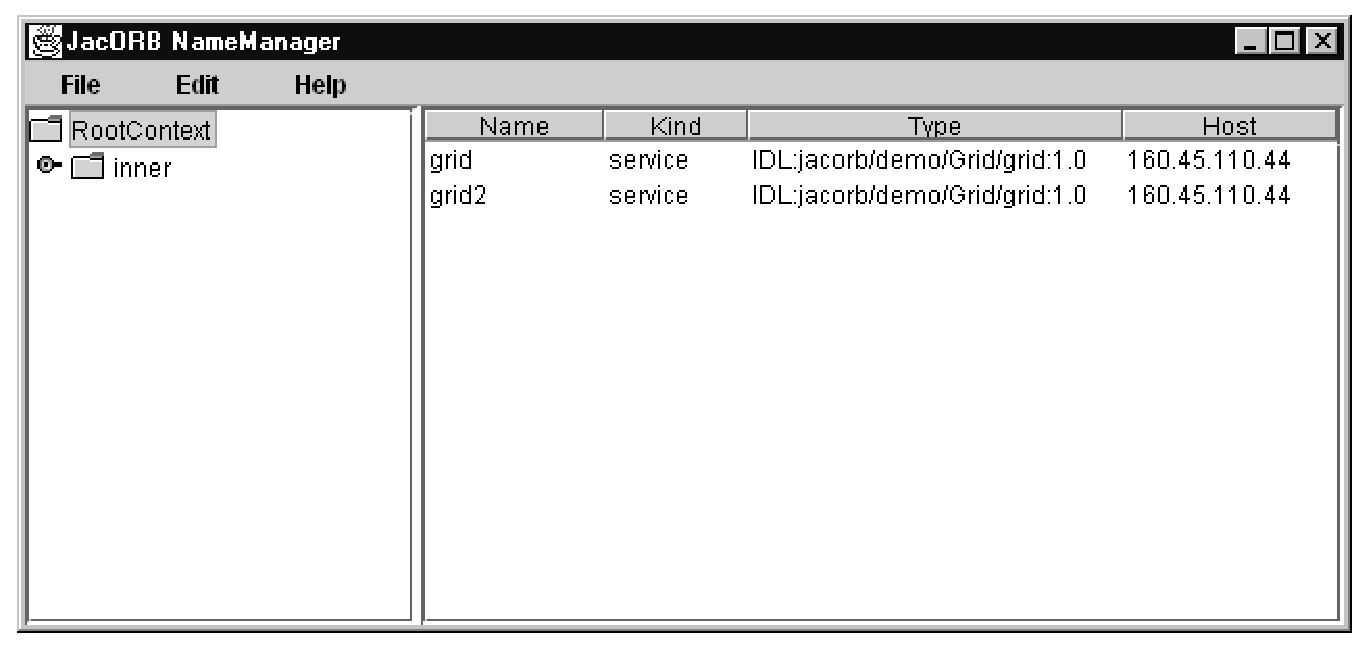
\epsfig{file=Nmgr1.eps, width=11cm}}
\caption{NameManager Screenshot}
\label{fig:nameManager}
\end{figure}

NameManager has menus  that let you unbind names  and create or delete
naming contexts within the root context. Creating a nested name space,
e.g., can be done by selecting the {\tt RootContext} and bringing up a
context  by clicking  the right  mouse button.  After  selecting ``new
context'' from that menu, you will be  prompted to enter a name for the
new, nested context.


%%%%%%%%%%%%%%%%%%%%%%%%%%%%%%%%%%%%%%%%%%%%%%%%%%%%%%%%%%%%%%%%%%%%%%%%%%%%%%

\chapter{The server side: POA, Threads}
\label{POA}

This  chapter   describes  the   facilities  offered  by   JacORB  for
controlling  how servers are  started and  executed. These  include an
activation daemon, the Portable Object Adapter (POA), and threading.

This chapter gives only a very superficial introduction to the POA.  A
thorough explanation of how the  POA can be used in different settings
and of the  different policies and strategies it  offers is beyond our
scope here,  but can be found in  \cite{Brose2001a}.  Other references
that  explain  the  POA  are  \cite{Henning1999,  Vinoski1998}.   More
in--depth  treatment in  C++ can  be found  in the  various C++-Report
Columns on the POA by  Doug Schmidt and Steve Vinoski.  These articles
are                            available                            at
\verb+http://www.cs.wustl.edu/~schmidt/report-doc.html+.  The ultimate
reference, of course, is the CORBA specification.

\section{POA}

The POA provides a comprehensive set of interfaces for managing object
references and servants. The code  written using the POA interfaces is
now portable across ORB implementations  and has the same semantics in
every ORB that is compliant to CORBA 2.2 or above.

The POA defines standard interfaces to do the following:
\begin{itemize}
\item Map an object reference to a servant that implements that object
\item Allow transparent activation of objects
\item Associate policy information with objects
\item  Make a  CORBA  object persistent  over  several server  process
lifetimes
\end{itemize}

In the POA specification, the use of pseudo-IDL has been deprecated in
favor  of an approach  that uses  ordinary IDL,  which is  mapped into
programming languages using the  standard language mappings, but which
is  locality constrained.  This means  that references  to  objects of
these types may not be passed outside of a server's address space. The
POA  interface  itself  is  one  example of  a  locality--constrained
interface.  

The  object adapter  is that  part of  CORBA that  is  responsible for
creating CORBA  objects and  object references and  --- with  a little
help  from  skeletons ---  dispatching  operation  requests to  actual
object  implementations.   In  cooperation  with   the  Implementation
Repository  it can also  activate objects,  i.e. start  processes with
programs that provide implementations for CORBA objects.

\section{Threads}

JacORB  currently  offers  one   server--side  thread  model.  The  POA
responsible for a given request will obtain a request processor thread
from  a central  thread pool.  The pool  has a  certain size  which is
always between the maximum and  minimum value configure by setting the
properties     {\tt     jacorb.poa.thread\_pool\_max}     and     {\tt
jacorb.poa.thread\_pool\_min}.

When a  request arrives and  the pool is  found to contain  no threads
because all  existing threads are  active, new threads may  be started
until     the    total    number     of    threads     reaches    {\tt
jacorb.poa.thread\_pool\_max}. Otherwise,  request processing is blocked
until a  thread is returned to  the pool. Upon  returning threads that
have  finished processing a  request to  the pool,  it must  be decided
whether  the  thread  should  actually   remain  in  the  pool  or  be
destroyed. If the current pool  size is above the minimum, a processor
thread will not be out into the pool again. Thus, the pool size always
oscillates between max and min.

Setting {\tt min} to a value  greater than one means keeping a certain
number  of   threads  ready  to  service   incoming  requests  without
delay. This is  especially useful if you now  that requests are likely
to come  in in a bursty fashion.  Limiting the pool size  to a certain
maximum  is  done to  prevent  servers  from  occupying all  available
resources.

Request  processor   threads  usually   run  at  the   highest  thread
priority. It is possible to influence thread priorities by setting the
property  {\tt jacorb.poa.thread\_priority} to  a value  between Java's
Thread.MIN\_PRIORITY and Thread.MAX\_PRIORITY. If the configured priority
value  is  invalid JacORB  will  assign  maximum  priority to  request
processing threads.




%%%%%%%%%%%%%%%%%%%%%%%%%%%%%%%%%%%%%%%%%%%%%%%%%%%%%%%%%%%%%%%%%%%%%%%%%%%%%%
\chapter{Implementation Repository}
\label{Ch_Imr}

\begin{quote}
``...  it is  very easy to be blinded to  the essential uselessness of
them by  the sense of achievement you  get from getting it  to work at
all.  In other  words --- and that is a  rock-solid principle on which
the whole of the Corporation's Galaxywide success is founded --- their
fundamental design  flaws are  completely hidden by  their superficial
design flaws.''
    
             D. Adams: So Long and Thanks for all the Fish
\end{quote}

The Implementation Repository is not, as its name suggests, a database
of  implementations.   Rather,  it  contains information  about  where
requests  to specific  CORBA objects  have  to be  redirected and  how
implementations  can be  transparently  instantiated if,  for a  given
request  to   an  object,  none  is   reachable.   ``Instantiating  an
implementation'' means starting a server program that hosts the target
object.  In  this  chapter  we  give  a brief  overview  and  a  short
introduction  on how to  use the  Implementation Repository.  For more
details please see \cite{Henning1999}.

\section{Overview}

Basically, the  Implementation Repository (ImR) is  an indirection for
requests  using  persistent  object  references. A  persistent  object
reference is one that was created  by a POA with a PERSISTENT lifespan
policy. This means that the lifetime of the object is longer than that
of its creating POA.   Using the Implementation Repository for objects
the lifetime  of which does not exceed  the life time of  its POA does
not make sense  as the main function of  the Implementation Repository
is to take care that such  a process exists when requests are made ---
and to start one if necessary.

To fulfill this function, the ImR  has to be involved in every request
to ``persistent  objects''.  This is achieved  by rewriting persistent
object  references to  contain {\em  not}  the address  of its  server
process but  the address  of the ImR.   Thus, requests  will initially
reach the ImR and not the actual server --- which may not exist at the
time of the request. If such a request arrives at the ImR, it looks up
the  server information  in its  internal tables  to determine  if the
target object is reachable or not.  In the latter case, the ImR has to
have  information  about how  an  appropriate  server  process can  be
started.   After   starting  this   server,  the  client   receives  a
LOCATION\_FORWARD  exception  from  the  ImR.  This  exception,  which
contains a new  object reference to the actual  server process now, is
handled by its runtime system  transparently.  As a result, the client
will automatically  reissue its request  using the new  reference, now
addressing the target directly.

\section{Using the JacORB Implementation Repository}

The  JacORB   Implementation  Repository  consists   of  two  separate
components:  a repository  process which  need  only exist  once in  a
domain, and  process startup daemons,  which must be present  on every
host that is  to start processes. Note that none  of this machinery is
necessary for processes that host  objects with a TRANSIENT life time,
such as used by the RootPOA.

First of all, the central repository process (which we will call ImR
in the following) must be started:

\cmdline{imr [-n] [-p <port>] [-i <ior\_file>][-f <file>][-b <file>] [-a]}

The   ImR   is  located   using   the   configuration  property   {\tt
jacorb.ImplementationRepositoryURL}.  This property  must be  set such
that  a  http  connection  can  be  made and  the  ImR's  IOR  can  be
read. Next, startup  daemons must be created on  selected hosts. To do
this, the following command must is issued on each host:

\cmdline{imr\_ssd}

When a startup  daemon is created, it contacts  the central ImR.

To register  a program such that  the ImR can start  it, the following
command is used (on any machine that can reach the ImR):

\cmdline{imr\_mg add "AServerName" -c "jaco MyServer"}

The {\tt imr\_mg} command is the  generic way of telling the ImR to do
something. It  needs another command  parameter, such as {\tt  add} in
this case. To add a server to the ImR, an {\em implementation name} is
needed. Here, it is {\tt  "AServerName"}.  If the host were the server
should be  restarted is not the  local one, use the  {\tt -h hostname}
option.  Finally, the  ImR needs to know how to  start the server. The
string {\tt "jaco  MyServer"} tells it how. The  format of this string
is simply such  that the server daemon can execute  it (using the Java
API call  {\tt exec()}), i.e.  it  must be intelligible  to the target
host's operating system.   For a Windows machine, this  could, e.g. be
{\tt "start jaco MyServer"} to have the server run in its own terminal
window, under Unix  the same can be achieved with  {\tt "xterm -e jaco
MyServer"}.

The startup  command is a  string that is  passed as the  {\em single}
argument to javas {\tt Runtime.exec()} method, without interpreting it
or adding  anything. Since {\tt  Runtime.exec()} has system--dependent
behaviour, the startup string has to reflect that. While for most unix
systems  it  is  sufficient  to  avoid shell--expansions  like  *  and
\verb+~+,  windows--based  systems  do   not  pass  the  string  to  a
commandline interpreter so a simple {\tt jaco MyServer} will fail even
if it works if directly typed in at the dos prompt. Therefore you have
to  ``wrap'' the  core  startup command  in  a call  to a  commandline
interpreter. On NT the following startup command will do the job: {\tt
cmd /c "jaco MyServer"}.  Please keep in mind that if you use the {\tt
imr\_mg} command  to set the startup  command, you have  to escape the
quotes so they appear inside of the resulting string.

If you don't  intend to have your server  automatically started by the
ImR     you      can     also     set      the     property     ``{\tt
jacorb.imr.allow\_auto\_register}'' or use the  {\tt -a} switch of the
ImR  process. If  this property  is  set, the  ImR will  automatically
create a new  entry for a server on POA activation,  if the server has
not been registered previously. In this case you don't have to use the
ImR Manager to register your server.

For a client program to be  able to issue requests, it needs an object
reference.  Up to  this  point,  we haven't  said  anything about  how
persistent object  references come into  existence. Reference creation
happens as usual, i.e. in the server application one of the respective
operations  on a  POA is  called.  For a  reference to  be created  as
``persistent'',  the POA  must  have been  created  with a  PERSISTENT
lifespan policy. This is done as in the following code snippet:

\small{
\begin{verbatim}
    /* init ORB and root POA */
    orb = org.omg.CORBA.ORB.init(args, props);
    org.omg.PortableServer.POA rootPOA = 
        org.omg.PortableServer.POAHelper.narrow(
                        orb.resolve_initial_references("RootPOA"));

    /* create policies  */

    org.omg.CORBA.Policy [] policies = new org.omg.CORBA.Policy[2];
    policies[0] = rootPOA.create_id_assignment_policy(
                                IdAssignmentPolicyValue.USER_ID);
    policies[1] = rootPOA.create_lifespan_policy(
                                LifespanPolicyValue.PERSISTENT);

    /* create POA */

    POA myPOA = rootPOA.create_POA("XYZPOA", 
                                rootPOA.the_POAManager(), policies);

    /* activate POAs */                              
    poa.the_POAManager().activate();

\end{verbatim}
}

(Note that in general the  id assignment policy will be {\tt USER\_ID}
for a POA with persistent object references because this id will often
be a key into  a database where the object state is  stored). If a POA
is created with this lifespan policy and the ORB property ``use\_imr''
is set, the ORB will try to  notify the ImR about this fact so the ImR
knows it doesn't need to start  a new process for requests that target
objects on this  POA.  To set the ORB policy,  simply set the property
{\tt  jacorb.use\_imr=on}.   The   ORB  uses  another  property,  {\tt
jacorb.implname}, as  a parameter for the  notification, i.e.~it tells
the  ImR  that a  process  using this  property's  value  as its  {\em
implementation name} is present. If  the server is registered with the
ImR, this property value has  to match the implementation name that is
used when registering.

The application  can set  these properties on  the command  line using
{\tt java -Djacorb.implname=MyName}, or in the code like this:

\small{
\begin{verbatim}
    /* create and set properties */
    java.util.Properties props = new java.util.Properties();
    props.setProperty("jacorb.use_imr","on");
    props.setProperty("jacorb.implname","MyName");

    /* init ORB  */
    orb = org.omg.CORBA.ORB.init(args, props);
\end{verbatim}
}

There are a few things  you have to consider especially when restoring
object state  at startup time or  saving the state of  your objects on
shutdown. It is important that, at startup time, object initialization
is complete when the object  is activated because from this instant on
operation calls  may come  in. The repository  knows about  the server
when the  first POA with  a PERSISTENT lifespan policy  registers, but
does not  forward object  references to clients  before the  object is
actually reachable. (Another, unreliable way to handle this problem is
to  increase the {\tt  jacorb.imr.object\_activation\_sleep} property,
so the repository waits longer for the object to become ready again.)

When the server shuts down,  it is equally important that object state
is saved by the time the last POA in the server goes down because from
this moment  the Implementation Repository regards the  server as down
and will start a new one upon requests.  Thus, a server implementor is
responsible for avoiding reader/writer problems between servers trying
to store and  restore the object state.  (One way of  doing this is to
use POA  managers to set  a POA to  holding while saving state  and to
inactive when done.)

Please keep in mind  that even if you don't have to  save the state of
your objects  on server shutdown  you {\em must} deactivate  your POAs
prior   to   exiting   your    process   (or   at   least   use   {\tt
orb.shutdown(\dots)} which  includes POA deactivation).  Otherwise the
ImR keeps the  server as active and will return  invalid IORs. In case
of  a  server crash  you  can use  the  command  {\tt imr\_mg  setdown
AServerName} to notify the ImR of the server termination.

\section{Server migration}

The  implementation  repository  offers  another  useful  possibility:
server migration.   Imagine the  following scenario: You  have written
your  server with  persistent  POAs,  but after  a  certain time  your
machine  seems   to  be   too  slow  to   serve  all   those  incoming
requests.  Migrating your  server to  a more  powerful machine  is the
obvious  solution.    Using  the  implementation   repository,  client
references do not contain addressing information for the slow machine,
so server migration can be done transparently to client.

Assuming  that you  added your  server to  the repository,  and  it is
running  correctly.  

\cmdline{imr\_mg add AServerName -h a\_slow\_machine -c "jaco MyServer"}

The first step is to {\em  hold} the server, that means the repository
delays all requests for that server until it is released again.

\cmdline{imr\_mg hold AServerName}

Now  your server  will not  receive  any requests  for its  registered
POAs. If you can't shut your server down such that it sets itself down
at  the repository,  i.e.~your POAs  are  set to  inactive prior  to
terminating the process, you can use

\cmdline{imr\_mg setdown AServerName}

to  do  that.   Otherwise  your  POAs  can't  be  reactivated  at  the
repository because they are still logged as active.

If you  want your  server to be  restarted automatically, you  have to
tell the repository the new host and maybe a new startup command.

\cmdline{imr\_mg edit AServerName -h the\_fastest\_available\_machine\\
-c "jaco MyServer"}

If your server can be restarted automatically, you now don't even have
to start it manually, but it is instead restarted by the next incoming
request.  Otherwise start it manually on the desired machine now.

The last step is to release  the server, i.e.~let all delayed requests
continue.

\cmdline{imr\_mg release AServerName}

By now your  server should be running on  another machine, without the
clients noticing.

\section{A Note About Security}
Using the imr can pose a major security threat to your system. Imagine
the following standard setup: an imr  is running on a machine, its IOR
file is placed in a directory where  it can be read by the web server,
and several  imr\_ssds are running  on other machines. An  attacker can
now  execute processes  on the  machines the  ssds are  running  on by
taking the following steps:
\begin{enumerate}
         \item  Setting  the  {\tt  jacorb.ImplementationRepositoryURL}
         property to the IOR file on your server.
         \item  Creating a new logical server with the desired command
           to execute as startup command on the desired host (where a
           ssd is running). This is the crucial point. The ssd calls
           {\tt Runtime.exec()} with the supplied string, and there
           is no way to check if the command does what it is supposed
           to do, i.e.~start a server.
         \item Start the server with the imr\_mg. The startup command
           of the server will b exec'd on the specified host.
\end{enumerate}

Now this should  not generally discourage you to use  the imr but show
you  that   there  are  risks,  which  can   be  reduced  significantly
nonetheless. There  are several ways  to encounter this threat  and we
don't consider this list to be complete:
\begin{enumerate}
        \item Try to control the distribution of the IOR file. Hiding
          it should not be considered here, because {\it security by
            obscurity} is generally a bad approach. Try to make use of
          file system mechanisms like groups and ACLs.
          \item Use a firewall which blocks of incoming traffic. Keep
            in mind that if the attacker is inside of your protection
            domain, the firewall won't help. It is also not that hard
            to write a Trojan that can tunnel those firewalls that
            block incoming traffic.
          \item Enforce SSL connections to the imr. This blocks all
            client connections that don't have a certificate signed by
            a CA of your choice. See chapter \ref{SSL} for more
            information.
\end{enumerate}
%%%%%%%%%%%%%%%%%%%%%%%%%%%%%%%%%%%%%%%%%%%%%%%%%%%%%%%%%%%%%%%%%%%%%%%%%%%%%%
\chapter{Interface Repository}
\label{ch:interface_repository}

Run--time  type information  in CORBA  is  managed by  the ORB's  {\it
Interface Repository}  (IR) component.  It allows  to request, inspect
and modify IDL  type information dynamically, e.g., to  find out which
operations an object supports. Some ORBs  may also need the IR to find
out whether  a given object's type  is a subtype of  another, but most
ORBs can do  without the IR by encoding this  kind of type information
in the helper classes generated by the IDL compiler.

In essence,  the IR is  just another remotely accessible  CORBA object
that offers  operations to retrieve  (and in theory also  modify) type
information.  Note that the  JacORB IR  is only  available if  you are
using JDK 1.2 or above.

\section{Type Information in the IR}

The  IR  manages  type   information  in  a  hierarchical  containment
structure that  corresponds to the structure of  scoping constructs in
IDL  specifications:   modules  contain  definitions   of  interfaces,
structures, constants  etc. Interfaces in turn  contain definitions of
exceptions, operations, attributes  and constants. Figure \ref{IR-fig}
illustrates this hierarchy.

\begin{figure}[htb]
\centerline{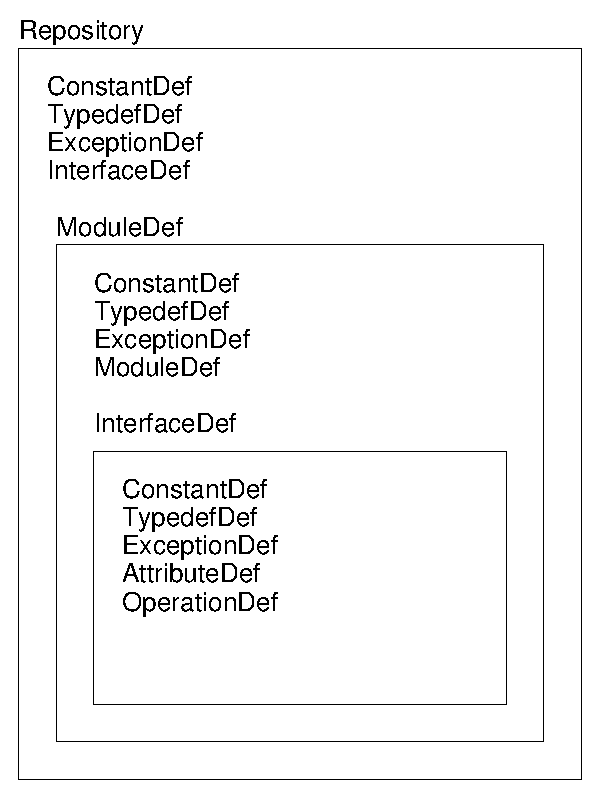
\epsfig{file=IR.eps, width=5cm}}
\caption{Containers in the Interface Repository}
\label{IR-fig}
\end{figure}

The  descriptions  inside  the  IR  can  be  identified  in  different
ways. Every  element of  the repository has  a unique,  qualified name
which  corresponds  to  the  structure  of  name  scopes  in  the  IDL
specification. An interface {\tt  I1} which was declared inside module
{\tt M2} which in turn was  declared inside module {\tt M1} thus has a
qualified name  {\tt M1::M2::I1}. The  IR also provides  another, much
more   flexible   way   of    naming   IDL   constructs   using   {\it
Repository Id}s.  There   are  a   number  of  different   formats  for
RepositoryIds  but  every  Repository  must  be  able  to  handle  the
following format, which is marked  by the prefix {\tt "IDL:"} and also
carries  a  suffix   with  a  version  number,  as   in,  e.g.,  "{\tt
IDL:jacorb/demo/grid:1.0}". The name  component between the colons can
be set freely using the  IDL compiler directives {\tt \#pragma prefix}
and {\tt \#pragma ID}. If no such directive is used, it corresponds to
the qualified name as above.

\section{Repository Design}

When designing the  Interface Repository, our goal was  to exploit the
Java reflection  API's functionality to  avoid having to  implement an
additional data base for  IDL type descriptions. An alternative design
is to use the IR as a back-end to the IDL compiler, but we did not want
to  introduce such  a  dependency and  preferred  to a  have a  rather
``light--weight'' repository  server.  As  it turned out,  this design
was  possible because  the similarities  between the  Java  and CORBA
object models allow  us to derive the required  IDL information at run
time. As  a consequence,  we can  even do without  any IDL  at compile
time.  In addition  to this simplification, the main  advantage of our
approach lies in avoiding  redundant data and possible inconsistencies
between  persistent IDL descriptions  and their  Java representations,
because Java classes have to be generated and stored anyway.

Thus, the  Repository has to  load Java classes, interpret  them using
reflection  and   translate  them   into  the  appropriate   IDL  meta
information. To  this end, the  repository realizes a  reverse mapping
from   Java   to  IDL.   Figure   \ref{IR-Process}  illustrates   this
functionality,  where $f^{-1}$  denotes  the reverse  mapping, or  the
inverse of  the language  mapping.

\begin{figure}[htb]
\centerline{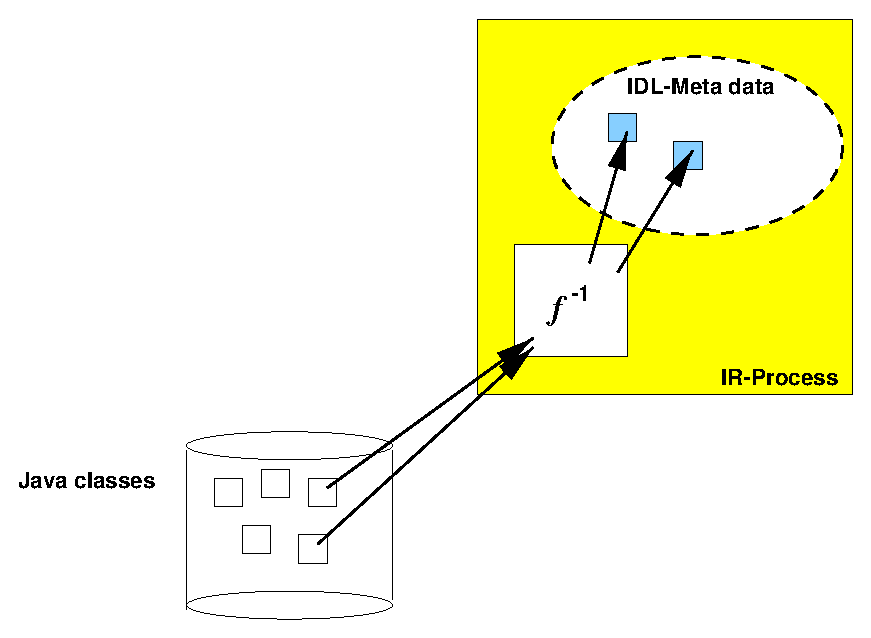
\epsfig{file=IR-Process.eps, width=7cm}}
\caption{The JacORB Interface Repository}
\label{IR-Process}
\end{figure}

\section{Using the IR}

For the ORB to be able to contact the IR, the IR server process must
be running. To start it, simply type the {\tt ir} command and provide
the required arguments:

\cmdline{ir /home/brose/classes /home/brose/public\_html/IR\_Ref}

The first  argument is  a path to  a directory containing  {\tt .class}
files and packages. The IR  loads these classes and tries to interpret
them as  IDL compiler--generated classes.  If it  succeeds, it creates
internal representations  of the  adequate IDL constructs.  The second
argument on  the command  line above  is simply the  name of  the file
where the IR stores its object reference for ORB bootstrapping.

To view the contents of the repository, you can use the GUI IRBrowser
tool or the query command. First, let's query the IR for a particular
repository ID. JacORB provides the command {\tt qir} (``query IR'')
for this purpose:

\cmdline{qir IDL:raccoon/test/cyberchair/Paper:1.0}

As result, the IR returns an InterfaceDef object, and {\tt qir} parses
this and prints out:

\begin{verbatim}
     interface Paper
     {
        void read(out string arg_0);
        raccoon::test::cyberchair::Review getReview(in long arg_0);
        raccoon::test::cyberchair::Review submitReview(
            in string arg_0, in long a rg_1);
        void listReviews(out string arg_0);
     };
\end{verbatim}

To start the IRBrowser, simply type

\cmdline{irbrowser}

Figure \ref{fig:IRBrowser} gives a screen shot of the IR browser.

\bigskip
\begin{figure}[htb]
\centerline{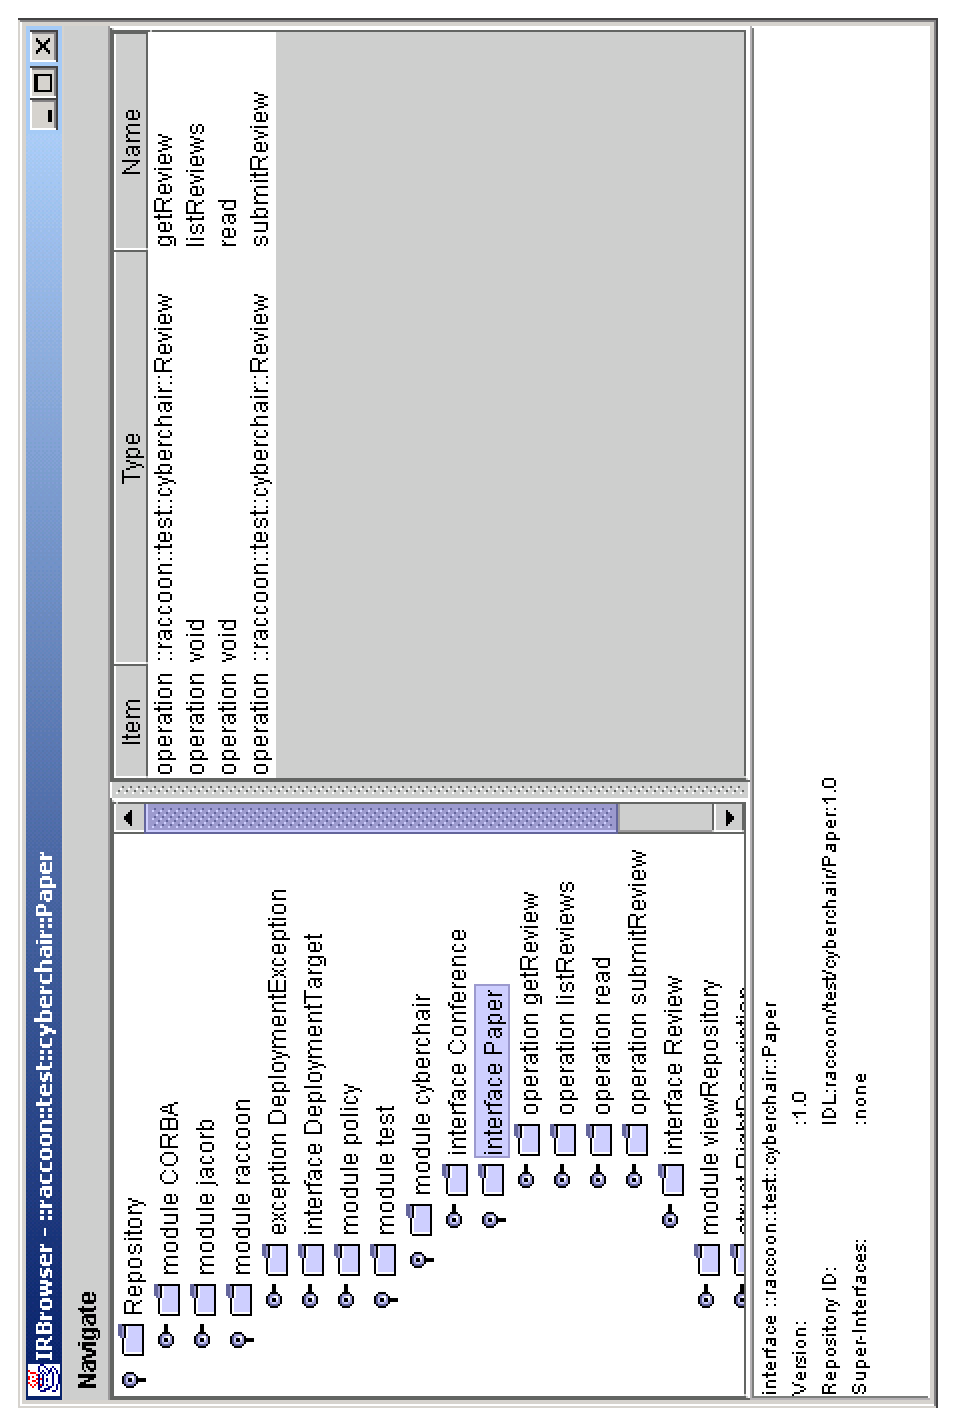
\epsfig{file=IRBrowser.eps, width=11cm, angle=270}}
\caption{IRBrowser Screenshot}
\label{fig:IRBrowser}
\end{figure}

The Java classes generated by  the IDL compiler using the standard OMG
IDL/Java language mapping do not contain enough information to rebuild
all  of the  information contained  in  the original  IDL file.   For
example,  determining whether an  attribute in  an interface  was {\tt
readonly} or  not is not  possible, or telling the  difference between
{\tt  in}  and {\tt  inout}  parameter  passing  modes. Moreover,  IDL
modules are not  explicitly represented in Java, so  telling whether a
directory in  the class  path represents an  IDL module is  not easily
possible. For these  reasons, the JacORB IDL compiler  generates a few
additional  classes that hold  the required  extra information  if the
compiler switch {\tt -ir} is used when compiling IDL files:

\cmdline{idl -ir myIdlFile.idl}

The additional files generated by the compiler are:
\begin{itemize}
\item a {\tt \_XModule.java} class file for any IDL module X
\item a {\tt YIRHelper.java} class file for any interface Y.
\end{itemize}

If no  {\tt .class} files that  are compiled from  these extra classes
are found  in the class path passed  to the IR server  process, the IR
will not  be able  to derive any  representations.  Note that  the IDL
compiler does not make any non--compliant modifications to any of the
standard files that are defined in the Java language mapping --- there
is only additional information.

One more caveat about these  extra classes: The compiler generates the
{\tt  \_XModule.java} class  only  for genuine  modules. Java  package
scopes created by applying the {\tt -d } switch to the IDL compiler do
not  represent   proper  modules  and   thus  do  not   generate  this
class. Thus, the contents of  these directories will not be considered
by the IR.

When an  object's client  calls the {\tt  get\_interface()} operation,
the ORB consults the IR  and returns an {\tt InterfaceDef} object that
describes the object's  interface. Using {\tt InterfaceDef} operations
on  this  description  object,  further  description  objects  can  be
obtained,  such as descriptions  for operations  or attributes  of the
interface under consideration.

The IR  can also be  called like any  other CORBA object  and provides
{\tt lookup()}  or {\tt lookup\_name()} operations to  clients so that
definitions can be searched for, given a qualified name. Moreover, the
complete contents of individual containers (modules or interfaces) can
be listed.

Interface   Repository  meta   objects  provide   further  description
operations. For a given {\tt  InterfaceDef} object, we can inspect the
different  meta   objects  contained   in  this  object   (e.g.,  {\tt
OperationDef} objects). It is  also possible to obtain descriptions in
form of a simple structure  of type {\tt InterfaceDescription} or {\tt
FullInterfaceDescription}. Since structures are  passed by value and a
{\tt   FullInterfaceDescription}    fully   provides   all   contained
descriptions,  no  further  ---possibly  remote  ---  invocations  are
necessary for searching the structure.


%%%%%%%%%%%%%%%%%%%%%%%%%%%%%%%%%%%%%%%%%%%%%%%%%%%%%%%%%%%%%%%%%%%%%%%%%%%%%%
\chapter{Applets --- The JacORB Appligator}
\label{Ch_applets}

{\em by Sebastian M{\"u}ller}

\bigskip
Since  version 1.0  beta  13,  JacORB includes  an  IIOP proxy  called
Appligator.  Using this proxy, you  can run Java Applets with JacORB.
Regular  java programs can  connect to  every host  on the  Internet ---
Applets can only  open connections to their applethost  (the host they
are downloaded  from).  This  lets Applets only  use CORBA  servers on
their applethost, if no proxy is used.  With JacORB Appligator, access
for your Applets  is no longer restricted.  Placed  on the applethost,
Appligator   handles  all   connections  from   and  to   your  applet
transparently.


\section{Using Appligator}

Due to the transparency of JacORB Appligator you can write your applet
as if it were  a normal CORBA program.  The only thing  you have to do
is to  use a special initialization of  the ORB: You have  to call the
{\tt     jacorb.orb.ORB(java.applet.Applet,     java.util.Properties)}
constructor.

A normal JacORB program reads  a local {\tt jacorb.properties} file to
get the URL of its name  server and other vital settings. An applet of
course has no {\em local} properties  file, but a remote one: You have
to place the properties file (which has the same syntax and parameters
as the  normal file) in  the same directory  as your applet  (the file
name has to be: {\tt jacorb.properties}, without a leading dot).

Similar to the name server, Appligator writes its IOR to a file.  Your
applet has  to know the location of  this file to retrieve  the IOR of
Appligator.   You  can  set the  location  of  the  IOR file  via  the
jacorb.properties  file (parameter  jacorb.ProxyServerURL) or  with an
applet    parameter   in    the   {\tt <APPLET>    HTML}    tag   (parameter
{\tt JacorbProxyServerURL}).  If  you give no (or a  wrong) parameter JacORB
will look for an IOR file called "proxy.ior" in the codebase directory
and in the web server root directory.

Make  sure  the  parameter  {\tt  jacorb.NameServerURL}  points  to  a
location on the applethost, otherwise  you will get an applet security
exception if your applet needs to use the name server.

\subsubsection*{Starting Appligator}

Just type  

\cmdline{appligator <port> <filename>} 

to  start the  proxy  on port  {\tt  port}.  {\tt  <filename>} is  the
location where the IOR of  the Appligator is written to. This location
has to be specified in the  jacorb.properties file of the applet or in
an  applet parameter  (if it  is not  one of  the standard  paths, see
below).

\subsubsection*{Summary}

\begin{itemize}
    \item init the  ORB with {\tt jacorb.orb.init(applet,properties)},
where   applet    is   this    applet   and   properties    are   {\tt
java.util.Properties} (which can be null)
        
    \item put a {\tt jacorb.properties} file in the directory of the applet

    \item specify the location for the appligator IOR file in the {\tt
jacorb.properties} (jacorb.ProxyServerURL)  or in an  applet parameter
(JacorbProxyServerURL)

    \item make sure the name server IOR file is accessible for the applet
      (lies on the applethost)

    \item  start Appligator  on  the applethost  (web server)  with:\\
\cmdline{appligator <filename>}\\  where filename is  the location the
appligator IOR is  put to and has to be the  location specified in the
jacorb\_properties or applet parameter.
\end{itemize}


\subsubsection*{Applet Properties}

As  described above  there are  some ways  for the  applet to  get its
jacorb  properties.  The  most important  property is  the URL  to the
appligator  IOR  file.  Without  this  property the  applet  will  not
work. If you use a name server,  the URL to the name server IOR has to
be specified too.

Properties can be set in three ways:
\begin{enumerate}
     \item   in  the  {\tt ORB.init()}  call  with  the  
     {\tt java.util.Properties}parameter
                 
     \item  in the {\tt  jacorb\_properties} file  located in  the same
     directory as the applet

     \item the URL  to the name server and Appligator  IOR file can be
     set in the applet tag in the HTML file
\end{enumerate}


\subsubsection*{Appligator and Netscape/IE, appletviewer}

Netscape  Navigator/Communicator comes with  its own  (outdated) CORBA
support. You have to delete Netscape's CORBA classes to use JacORB. To
do  this  you have  to  delete the  file  iiop10.jar  located in  {\tt
NS\_ROOT/java/classes}.   It's  a  good  idea  to store  a  backup  of
Netscape's file in another directory. Note that renaming this jar file
in the original directory does  not suffice if you don't also change
the {\tt .jar} extension because  Netscape loads all jar files in this
directory. You then need to install jacorb.jar in this directory.

If Netscape loads wrong classes  or throws security exceptions (have a
look at  Netscape's JAVA Console  to see this)  be sure to  check your
{\tt CLASSPATH} and look for old or .  Remove all JacORB  and VisiBroker classes  from your
{\tt CLASSPATH}. We succeeded running JacORB applet clients on
Netscape 4.72 with the Java 1.3 plugin.

Microsoft's  Internet   Explorer  is  stricter   than  Netscape:  Even
downloaded classes are not allowed  to listen on a socket. We strongly
advise to  use Sun's Java  1.3 plugin with  IE also. To trick  IE into
using   JacORB,   you   need   to   copy  JacORB   classes   to   {\tt
\$WINNT\\Java\\TrustLib}.  You can either  copy the  entire jacorb.jar
and  unpack it in  this directory  or just  copy the  directories {\tt
jacorb}, {\tt org}, and {\tt HTTPClient}.

Appligator works well  with Sun's appletviewer. You only  have to make
the  appletviewer  replace  the  Sun's  CORBA  classes  with  JacORB's
classes.  A  typical appletviewer call  for JacORB Applets  looks like
this (written in one command line):

\cmdline{appletviewer http://www.example.com/CORBA/dii\_example.html}

There is a shell script  called "jacapplet" in JacORB's bin directory,
which calls the appletviewer with the appropriate options (you have to
edit it to match your local jdk path).

If you use the Appligator with other browsers or if you know a 
way to load the JacORB classes without removing and copying jars please 
let us know.

\subsubsection*{Examples}

There  are   some  example  applets   in  the  demo   directory  ({\tt
jacorb/demo/applet}).   They are  based on  the normal  examples.  The
examples  include a  HTML file  which calls  the applet.   To  run the
example  start the  name server  first. Start  appligator on  your web
server and than the normal  example server corresponding to the applet
example on any  computer in any order.  Then you  can call the example
applet with the JDK appletviewer or Netscape.

Be  sure  to  have  a   {\tt  jacorb.properties}  file  and  the  {\tt
jacorb.jar} in place.


\section{Using JacORB with Firewalls}

Typically firewalls do two things:  filter traffic by port, and filter
traffic  by protocol.   JacORB comes  with two  utilities  to overcome
firewall filtering.   The JacORB Appligator  can be used to  deal with
port  restrictions, and  HTTP tunneling  helps you  to  tunnel through
firewalls that are blocking GIOP messages.


\subsection{The JacORB Appligator}

The Appligator was written to  avoid the sandbox restrictions for Java
applets. Unsigned applets  can only have connections to  the host they
are loaded  from, which makes  them useless in most  distributed CORBA
scenarios. The  Appligator is a  GIOP proxy, which enables  applets to
connect  to every  CORBA server  by redirecting  the traffic  from the
applet to the CORBA server to the proxy. The Appligator also works the
other  way round:  Every connection  the applet  is redirected  to the
Appligator.

Even without applets  the Appligator can be used as a  GIOP proxy on a
firewall. The  Appligator is a  CORBA object itself and  is explicitly
started  on   a  given  port  using  a   command--line  argument  {\tt
<portnumber>}.  All incoming traffic to the Appligator will go to port
{\tt  <portnumber>}.  If you  configure your  CORBA object  behind the
firewall to  be aware of the  Appligator all traffic from  and to this
objects  will go  through the  Appligator (a  better way  would  be to
distinguish between traffic going over the firewall and traffic within
the  enclave, this has  to be  implemented in  future versions  of the
Appligator).

To  make your  port filtering  firewall  working with  CORBA and  GIOP
messages you must  ask your system administrator to  assign a port for
GIOP messages on the firewall. Start the Appligator on this port.

Now  all CORBA servers  (which are  aware of  the Appligator)  in your
enclave can  be contacted over  the Appligator.  If your  CORBA client
wants to  contact a  server in the  Internet outside the  firewall the
connection will go over the Appligator. Callbacks from the Internet to
your client do not work with Netscape.

To make your  non--Applet clients and your CORBA  objects aware of the
Appligator you  have to add  a property in your  jacorb.property file.
Applets  will  use the  Appligator  automatically.  If  you want  your
applications to use  the Appligator (which is true if  you want to use
the     Appligator     as    a     firewall     proxy)    than     set
{\tt jacorb.use\_appligator\_for\_applications  = on}.  If  you want  to turn
off appligator use  set {\tt jacorb.use\_appligator\_for\_applications = off}
for  applications and  {\tt jacorb.use\_appligator\_for\_applets  = off}  for
applets.

Finally you  have to specify the  location on the  Appligator. This is
done the same way as  JacORB determines to location of the name server:
When the Appligator  starts the IOR of the Appligator  is written to a
file which is put to  the location you specified as command parameter.
This  file must  be accessible  to all  clients that  want to  use the
Appligator.  You  can use a shared  file system to access  this file or
put it on a web server etc.  The location of the file in which the IOR
of  the Appligator  is stored  must  be set  in the  jacorb.properties
file. Use the "jacorb.ProxyServerURL" property for this.


\subsection{HTTP tunneling}

If your firewall filters traffic  by protocol and is not configured to
allow  GIOP messages  you can  use HTTP  tunneling to  make  your GIOP
traffic look  like HTTP traffic to  the firewall. HTTP  tunneling is a
built--in feature of  JacORB and produces correct HTTP  1.1 messages so
that your firewalls sees a HTTP request (from your CORBA client to the
CORBA server) and a HTTP reply  (from the CORBA server to your client)
for each method  you call on the server.  

HTTP tunneling in JacORB is not compatible with any OMG standard so it
will  work between  JacORB  clients and  servers  only.  Every  JacORB
server  will  recognize  incoming  HTTP  traffic and  will  handle  it
correctly without  any special settings needed.   Configuration has to
be done on the client side.   You can configure HTTP tunneling on a IP
address basis.  If  you set HTTP tunneling on for  a given IP address,
all traffic will  be tunneled to all CORBA objects  on this host.  You
can specify more than one IP  address by using a comma separated list.
Example:If you set  {\tt jacorb.use\_httptunneling\_for = 192.168.0.1,
192.168.0.2}  all  traffic  to  192.168.0.1 and  192.168.0.2  will  be
tunneled.


\subsection{Appligator and tunneling}

As  the  Appligator  is  a  normal JacORB  CORBA  object  it  supports
tunneling,  too.   No  extra   configuration  is  needed  to  use  the
Appligator on a firewall and tunnel the firewall with HTTP.

\subsection{Summary}

\begin{itemize}
\item  use the  Appligator as  a GIOP  proxy an  the firewall  if your
firewall  is configured  to  block  all traffic  but  traffic on  some
special ports.

\item ask your system administrator  to assign a special port for GIOP
on  your  firewall  and start  the  Appligator  on  this port  on  the
firewall: for example

\cmdline{appligator 7777 Appligator\_Ref}

\item  all CORBA  objects that  should be  reachable from  outside the
firewall or need  to contact a CORBA object  outside the firewall must
use    the     Appligator    as     a    proxy.    Add     the    {\tt
jacorb.use\_appligator\_for\_applications   =  on}  property   to  the
jacorb.properties file for those applications

\item Set the location of the Appligator in the jacorb.properties file
of your clients ({\tt jacorb.ProxyServerURL})

\item If you need HTTP  tunneling because a firewall between your host
and  server   is  filtering  GIOP  messages  use   the  property  {\tt
jacorb.use\_httptunneling\_for} with the IP  address of the server you
want to use tunneling to

\end{itemize}


\subsection*{Final remarks}

I want to thank Wendell Duncan for testing and debugging the tunneling
code.  I do not have a real firewall here in university, so I hope all
the stuff works  in a real environment :-). If  you have problems feel
free to contact  me.  I would be glad to hear  if you successfully use
the Appligator or HTTP tunneling.


%%%%%%%%%%%%%%%%%%%%%%%%%%%%%%%%%%%%%%%%%%%%%%%%%%%%%%%%%%%%%%%%%%%%%%%%%%%%%%

\chapter{IIOP over SSL}

\label{SSL}

Using  SSL to authenticate  clients and  to protect  the communication
between client and target requires no changes in your source code. The
only  notable  effect  is  that  SSL/TLS type  sockets  are  used  for
transport  connections  instead of  plain  TCP  sockets  --- and  that
connection setup takes a bit longer.

The only  prerequisites are that you rebuild  JacORB with cryptography
support. You  also need  to set up  a key  store file that  holds your
cryptographic   keys,  and  to   configure  SSL   by  setting   a  few
properties. All of this is described in this chapter.

\section{Re--Building JacORB's security libraries}

In the  standard distribution, the  JacORB security libraries  are not
enabled.   To do  so, you  simply need  to recompile  JacORB  with the
required SSL and JCE libraries  in your CLASSPATH.  If these libraries
are not found, JacORB will be rebuilt without SSL support.

To  successfully rebuild  JacORB with  SSL support,  the  following is
required:

\begin{itemize}
        \item JDK 1.2 or later,

        \item   IAIK-JCE   2.591,   the  security   provider   classes
downloadable from \\ {\tt http://jcewww.iaik.tu-graz.ac.at/},

     \item iSaSiLk 3.0 or later,  the SSL implementation from the same
source.\footnote{We   will   allow   using   SUN  provider   and   SSL
implementation in a future release}
\end{itemize}

Make  sure that  the two  libraries are  in your  CLASSPATH. Then build
JacORB anew by typing {\tt ant} in your JacORB installation directory.

\section{Setting up a key store}

SSL  relies   on  public  key  certificates  in   the  standard  X.509
format. These  certificates are presented in  the authentication phase
of the  SSL handshake and used  to compute and  exchange session keys.
This section explains how to create and store these certificates.

The Java 2  security API provides interfaces that  access a persistent
data structure  called {\em  KeyStore}. A key  store is simply  a file
that contains  public key  certificates and the  corresponding private
keys. It also  contains other certificates that can  be used to verify
public key  certificates.  All  cryptographic data is  protected using
passwords and accessed using names called {\em aliases}.

JacORB provides a  GUI tool to create and  manipulate key store files,
the  KeyStoreManager. It  can generate  key pairs,  sign  public keys,
import  or   export  certificates,  and   define  trusted  certificate
authorities. To start the KeyStoreManager, simply type {\tt ks} on the
command  line. The GUI  lets you  select and  open existing  key store
files, or create new ones.

Starting with an  empty key store, you first need to  create a new key
store and then  a key pair and certificate. Select  {\tt New} from the
{\tt File}  menu to create  a key store,  and then {\tt New}  from the
{\tt Keys} menu.   You will then be asked to provide  a new alias name
for your  new key entry. You also  need to choose a  password. You can
leave  the  algorithm  and  key  length fields  in  the  combobox  menu
unchanged.

\bigskip
\centerline{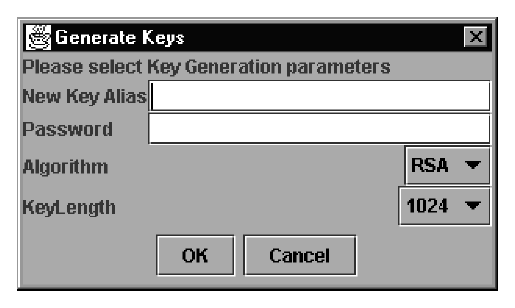
\epsfig{file=Generate.eps, width=7cm}}

You  now  have a  public  key certificate  that  you  can present  for
authentication, claiming  identity with the  alias name that  has been
embedded  in the  certificate.   Since anybody  could  present such  a
certificate,  receivers  require  that  the certificate  be  digitally
signed by someone  they trust, a {\em Certificate  Authority} (CA). By
signing  the certificate,  a CA  supports  the identity  claim of  the
certificate  subject. Whose  signature is  accepted as  trustworthy is
just a matter  of configuration, but normally proper  CAs are expected
to only sign certificates that  they have carefully scrutinized --- or
even created themselves. 

\bigskip
\centerline{\epsfig{file=Keystore.eps, width=11cm}}

For   convenience  you   can  act   as  a   CA  yourself,   using  the
KeyStoreManager GUI  to import certificates  and then sign  and export
them  again.   The  originating  key  store can  then  re--import  the
certificate that now bears the  digital signature of someone acting as
a CA. The key store has a  standard key chain format that must be used
to store public key certificates. The  first entry in the key chain is
your own public  key certificate as generated by the  key store. It is
automatically signed with its own  private key. Second in the chain is
the public key certificate that is signed by the CA. The last entry in
a key  chain must hold the  CA's public key  certificate, signed using
its private key. Trust in the CA key is ``axiomatic''. 

\bigskip
\centerline{\epsfig{file=KSMenu.eps, width=11cm}}

You can  check the validity of a  key chain by selecting  an alias and
then choosing {\tt Verify Chain}  from the {\tt Keys} menu. Unless the
key  chain  has  the proper  format  {\em  and}  the CA's  public  key
certificate is also declared  as trusted using the {\tt Trustees--add}
menu, the  verification will fail.  Only of  the verification succeeds
will you be able to use a public key certificate in the SSL connection
setup. More documentation on key stores  can be found in the Java tool
documentation for the {\tt keytool}  command. If you care for ``real''
security,  be advised  that setting  up  and managing  (or finding)  a
properly administered CA is essential for the overall security of your
system.

Finally,  note that  key  stores  are normally  used  only for  client
authentication in JacORB.   Servers may, but need not,  have their own
keys and  passwords because server authentication is  optional and not
mandatory like  client authentication. Technically,  this is achieved
by  exchanging the  client  and server  roles  at SSL  setup. This  is
entirely  transparent to  applications, of  course, but  might prevent
interoperation  with other ORBs  over SSL  if their  SSL setup  is not
prepared to handle this role change.

\subsection{Step--By--Step certificate creation}
In  order to  generate  a  simple public  key  infrastructure you  can
perform the following steps:
\begin{enumerate}
\item Create new keystores (File/new) and keypairs (Keys/new) for the CA
and for the user.
\item  Open the  user keystore (File/open),  select the  key  entry and
export the self-signed certificate (Certificates/Export).
\item  Open  the  CA  keystore  and  add the  user  certificate  as  a
Trustee (Trustees/add\dots).
\item Select the  trusted user certificate and create  a signed public
key certificate (Certificates/Create). Leave the role name field empty,
enter the  CAs private  key password and  save the new  certificate by
clicking OK.
\item Export the  CAs self-signed certificate to a  file (as explained
above).    Delete    the    trusted    certificate   from    the    CA
keystore (Trustees/Delete).
\item Open the  user keystore again. Select the  key entry, the import
the CA-signed  user cert (Certificates/Import), and  the self-signed CA
cert.
\item Add  the self-signed CA cert  as a trustee. This  is only needed
for verifying the chain, therefor the keystore can be deployed without
it.  Please  note  that  a  failed  verification  might  result  in  a
SignatureException.
\end{enumerate}

\section{Configuring SSL properties}

When the ORB is initialized by the application, a couple of properties
are read from files and the  command line. For the default SSL support
we define two properties:

\begin{verbatim}
        jacorb.security.support_ssl=on
        jacorb.security.enforce_ssl=on    
\end{verbatim}

If {\tt  enforce\_ssl} is  on, your application  requires that  SSL be
used  for  all  its  connections,  both incoming  and  outgoing.  {\tt
CORBA::NO\_PERMISSION} is  thrown if the  policy is violated.  If your
application is  a server,  you can thus  use SSL to  authenticate your
clients and,  in more  advanced scenarios using  interceptors, perform
operation--based access control. As  a client, you would probably only
require  SSL if  you are  careful to  protect your  communication from
eavesdropping or tampering.

The {\tt support\_ssl} option is  used if you don't require protection
yourself but  are prepared to use  SSL if the other  side requires it.
If {\tt  support\_ssl=off} then {\tt enforce\_ssl=off}  also.  If {\tt
jacorb.security.support\_ssl=on}  the user  will have  to authenticate
himself. To  be able  to provide the  required certificates,  the user
will have to provide the key store alias and a password to the ORB.

These SSL settings can be further refined using security options as in
the following property definitions:

\begin{verbatim}
        jacorb.security.ssl.supported_options=40
        jacorb.security.ssl.required_options=0
\end{verbatim}

The  value  of  these security  options  is  a  bit  mask coded  as  a
hexadecimal integer. The meanings of the individual bits is defined in
the CORBA Security Service  Specification and reproduced here from the
{\tt Security.idl} file:

\begin{verbatim}
        typedef unsigned short   AssociationOptions;

        const AssociationOptions NoProtection = 1;
        const AssociationOptions Integrity = 2; 
        const AssociationOptions Confidentiality = 4; 
        const AssociationOptions DetectReplay = 8; 
        const AssociationOptions DetectMisordering = 16;
        const AssociationOptions EstablishTrustInTarget = 32; 
        const AssociationOptions EstablishTrustInClient = 64;
        const AssociationOptions NoDelegation = 128;
        const AssociationOptions SimpleDelegation = 256; 
        const AssociationOptions CompositeDelegation = 512;
\end{verbatim}

With the  current SSL integration  in JacORB, the only  valid settings
are  EstablishTrustInTarget  and/or  EstablishTrustInClient, i.e.  hex
values 40 or 60. NoProtection is not possible when SSL is used. If you
don't want protection, switch SSL support off.

As explained  in the previous  section, cryptographic data  (key pairs
and  certificates) is  stored in  a  keystore  file. To configure the
file name of the keystore file, you need to define the following
property:

\begin{verbatim}
        jacorb.security.keystore=AKeystoreFileName
\end{verbatim}

To avoid  typing in  lots of  aliases and passwords  (one for  the key
store, and  one for each entry  that is used), you  can define default
aliases and passwords like this:

\begin{verbatim}
# the name of the default key alias to look up in the keystore
jacorb.security.default_user=brose
jacorb.security.default_password=jacorb

# the name and location of the keystore relative to the home directory
jacorb.security.keystore=.keystore
\end{verbatim}

%%%%%%%%%%%%%%%%%%%%%%%%%%%%%%%%%%%%%%%%%%%%%%%%%%%%%%%%%%%%%%%%%%%%%%%%%%%%%%

\chapter{Portable Interceptors}

Since revision  1.1 JacORB provides support  for Portable Interceptors
These  interceptors are compliant  to the  specification which  can be
found  at  http://cgi.omg.org/cgi-bin/doc?ptc/00-03-03.  Therefore  we
don't  provide any  documentation on  how to  program  interceptors but
supply a  few (hopefully  helpful) hints and  tips on  JacORB specific
solutions.

The first  step to have an  interceptor integrated into the  ORB is to
register an {\em  ORBInitializer}. This is done by  setting a property
the following way:
\begin{verbatim}org.omg.PortableInterceptor.ORBInitializerClass.<any_suffix>=
   <orb initializer classname>
\end{verbatim}
The suffix  is just to distinguish between  different initializers and
doesn't have to  have any meaningful value. The  value of the property
however has to be the fully qualified classname of the initializer. If
the  verbosity  is  set  to  $\geq  2$  JacORB  will  display  a  {\tt
ClassNotFoundException} in  case the initializers class is  not in the
class path. 

An example line might look like:
\begin{verbatim}org.omg.PortableInterceptor.ORBInitializerClass.my_init=  
   test.MyInterceptorInitializer
\end{verbatim}

Unfortunately the  interfaces of  the specification don't  provide any
access to  the ORB.  If  you need  access to the  ORB from out  of the
initializer  you  can  cast  the  {\tt  ORBInitInfo}  object  to  {\tt
jacorb. orb.portableInterceptor.ORBInitInfoImpl}   and   call  {\tt
getORB()}  to  get  a  reference  to the  ORB  that  instantiated  the
initializer.

When working with service contexts please make sure that you don't use
{\tt  java.lang.Integer. MAX\_VALUE}  as an  id  because a  service
context with  that id  is used internally.  Otherwise you will  end up
with  either   your  data   not  transfered  or   unexpected  internal
exceptions.


%%%%%%%%%%%%%%%%%%%%%%%%%%%%%%%%%%%%%%%%%%%%%%%%%%%%%%%%%%%%%%%%%%%%%%%%%%%%%%

\chapter{JacORB utilities}

In this chapter, we will briefly explain the executables that come
with JacORB. These include the IDL--compiler, the JacORB name server.


\section{idl}

The IDL compiler parses IDL specifications  and maps these to a set of
Java classes. IDL interfaces  are translated into Java interfaces, and
typedefs,   structs,   const  declarations   etc.   are  mapped   onto
corresponding Java  classes.  Using {\tt idl},  stubs and
skeletons  for  all interface  types  in  the  IDL specification  will
automatically be generated.

\subsection*{Usage}

\noindent{\tt idl
  [-h|-help] [-v|-version] [-syntax] [-all] [-Idir] [-Dsymbol[=value]]
  [-d <Output Dir>] [-p <package\_prefix>] [-i2jpackage <mapping>][-W debug\_level]   <filelist>}

The option {\tt  -v} prints out a short version  string while {\tt -h}
or {\tt -help} displays brief usage information.

The {\tt -noskel} option suppresses the generation of skeleton files,
which may be unnecessary if you only want to {\em use} a reference and
thus need client--side code.

The  {\tt -ir} option  instructs the  compiler to  generate additional
files   that    contain   information   needed    by   the   Interface
Repository. Basically, there  is one (very small) extra  file for each
IDL module, and another additional file per IDL interface.

Invoking {\tt idl}  with the {\tt -syntax} option  allows you to check
your IDL  specification for  syntactic errors without  producing code.
Without {\tt  -syntax}, the compiler creates  directories according to
the Java package structure. 

The  compiler  does  not,  by  default,  generate  code  for  included
files. If that is desired, you have to use the {\tt -all} option which
causes code to be generated  for every IDL file directly or indirectly
included from within  {\tt <filelist>}. If you want  to make sure that
for a given IDL no code will  be generated even if this option is set,
you  can use  the  (proprietary) preprocessor  directive {\tt \#pragma
inhibit\_code\_generation}.

The {\tt-I} options allows you to specify one or more search paths for
IDL files included from within  {\tt <filelist>}. If no path is given,
only the  current directory will  be considered. 

With the  {\tt -D} option you can  define symbols that can  be used by
the  preprocessor while  processing  the  IDL file.   If  no value  is
specified, the  symbol will be  defined with a  value of 1. The {\tt
  -U} option lets you undefine symbols again.

Compiling a  file with  a module {\tt  ModuleX} and an  interface {\tt
  InterfaceY} in it  will result in a subdirectory  {\tt ModuleX} with
  {\tt    InterfaceY.java}   in   it    (and   possibly    more   {\tt
  .java}--files). By default, the root  directory for all of the files
  created  during  the process  is  the  current  directory. You  can,
  however, provide a  different directory in which these  files are to
  be placed by  using the -d option. Using the -d  option when you are
  only checking the syntax of an IDL file has no effect.

With the  {\tt -p}  option it  is also possible  to specify  a package
prefix for the generated Java  classes. E.g., if the IDL file contains
a module {\tt Bank} which  defines an interface {\tt Account}, you can
direct   the   IDL   compiler    to   generate   Java   classes   {\tt
example.Bank.Account} by compiling with the package prefix set to {\tt
example}, i.e. by compiling with

\cmdline{idl -p example bank.idl}

The IDL compiler will create the appropriate directories if necessary.
Note that the effect is the same as if the entire contents of the IDL
file was scoped with {\tt example}. In particular, this applies to
included files: all definitions in included files will also be scoped
this way! The -p switch should used with discretion in cases where
other IDL files are included.

To be able to flexibly redirect generated Java classes into packages,
the {\tt -i2jpackage} switch can be used. Using this option, any IDL
scope x can be replaced by one (or more) Java packages y. Specifying
{\tt -i2jpackage X:a.b.c} will thus cause code generated for IDL
definitions within a scope x to end up in a Java package {\tt a.b.c},
e.g. an IDL identifier {\tt X::Y::ident} will be mapped to {\tt
  a.b.c.y.ident} in Java.

(The  IDL  parser  was   generated  with  Scott  Hudson's  CUP  parser
generator.  The  LALR grammar for  the CORBA IDL  is in the  file {\tt
jacorb/Idl/parser.cup}.)

\section{ns}

JacORB provides a service for mapping names to network references. The
name server itself is written in Java like the rest of the package and
is a  straightforward implementation  of the CORBA  ``Naming Service''
from  Common  Object Services  Spec.,  Vol.1  \cite{OMG1997}. The  IDL
interfaces are mapped to Java according to our Java mapping.

\subsection*{Usage}

\cmdline{ns <filename>  [<timeout>]}

or 

\cmdline{jaco jacorb.Naming.NameServer <filename>  [<timeout>]}

\subsection*{Example}

\cmdline{ns \~/public\_html/NS\_Ref}

The name server does {\it not}  use a well known port for its service.
Since clients  cannot (and  need not) know  in advance where  the name
service will  be provided, we use  a bootstrap file in  which the name
server records  an object reference to itself  (its {\it Interoperable
Object Reference} or  IOR). The name of this bootstrap  file has to be
given as an argument to the  {\tt ns} command. This bootstrap file has
to  be available  to clients  network-wide, so  we demand  that  it be
reachable  via a  URL  --- that  is,  there must  be an  appropriately
configured HTTP server in your network domain which allows read access
to the bootstrap  file over a HTTP connection.  (This implies that the
file must have its read  permissions set appropriately. If the binding
to the name service fails, please  check that this is the case.) After
locating the name service through this mechanism, clients will connect
to the name server directly, so the only HTTP overhead is in the first
lookup of the server.

The name bindings in the server's database are stored in and retrieved
from a file that is found in the current directory unless the property
{\tt jacorb.naming.db\_dir} is set to a different directory name. When
the server  starts up, it tries  to read this file's  contents. If the
file  is  empty or  corrupt,  it will  be  ignored  (but overridden  on
exit). The name server can only save its state when it goes down after
a specified timeout. If the server is interrupted (with {\tt CTRL-C}),
state information  is lost  and the file  will not contain  any usable
data.

If no timeout is specified, the name server will simply stay up until
it is killed. Timeouts are specified in milliseconds.

\section{nmg}

The JacORB  NameManager, a  GUI for the  name service, can  be started
using the {\tt nmg} command.  The NameManager then tries to connect to
an existing name service.

\subsection*{Usage}

\cmdline{nmg}

\section{lsns}

This utility  lists the contents  of the default naming  context. Only
currently active servers that have registered are listed. The {\tt -r}
option recursively lists the  contents of naming contexts contained in
the root  context. If  the graph of  naming contexts  contains cycles,
trying to list the entire contents recursively will not return...

\subsection*{Usage}


\cmdline{lsns [-r] }

\subsection*{Example}

\cmdline{lsns \\
\ /grid.service}

when only the server for the grid example is running and registered
with the name server.


\section{dior}

JacORB comes with a simple utility to decode an interoperable object reference
(IOR) in string form into a more readable representation. 

\subsection*{Usage}

\cmdline{dior <IOR-string> | -f <filename>}

\subsection*{Example}

In the following example we use it to print out the contents of the
IOR that the JacORB name server writes to its file:

\cmdline{dior -f \~/public\_html/NS\_Ref}
\small{\begin{verbatim}
------IOR components-----
TypeId  :       IDL:omg.org/CosNaming/NamingContextExt:1.0
Profile Id   :  TAG_INTERNET_IOP
IIOP Version :  1.0
Host    :       160.45.110.41
Port    :       49435
Object key :    0x52 6F 6F 74 50 4F 41 3A 3A 30 D7 D1 91 E1 70 95 04 
\end{verbatim}
}

\section{pingo}

``Ping'' an object using its stringified IOR. Pingo will call {\tt
  \_non\_existent()} on the object's reference to determine whether
  the object is alive or not.

\subsection*{Usage}

\cmdline{pingo <IOR-string> | -f <filename> }

\section{ir}

This command starts the JacORB Interface Repository, which is explained in
chapter \ref{ch:interface_repository}.

\subsection*{Usage}

\cmdline{ir <reppository calss path> <IOR filename> }

\section{qir}

This command queries the JacORB Interface Repository and prints out
re--generated IDL for the repository item denoted by the argument
repository ID.

\subsection*{Usage}

\cmdline{qir <reppository Id> }

\section{ks}

This command starts the JacORB KeyStoreManager, which is explained in
chapter \ref{SSL}

\subsection*{Usage}

\cmdline{ks}

%%%%%%%%%%%%%%%%%%%%%%%%%%%%%%%%%%%%%%%%%%%%%%%%%%%%%%%%%%%%%%%%%%%%%%%%%%%%%%

\chapter{Limitations, Feedback}

A few limitations and known bugs (list is incomplete):

\begin{itemize}
    \item the IDL compiler does not support 
    \begin{itemize}
        \item the {\tt context} construct
    \end{itemize}
    \item the API documentation and this document are incomplete.
\end{itemize}

\subsection*{Feedback and bug reports}

Please mail bug reports as well as criticism and experience reports to:

\verb+brose@inf.fu-berlin.de+

%%%%%%%%%%%%%%%%%%%%%%%%%%%%%%%%%%%
{
\bibliography{./guide}
\bibliographystyle{alpha}
}

\end{document}
